
\chapter{Week4}

\section{Wednesday}\index{week4_Friday_lecture}
This lecture will talk about the applications of Baire-Category Theorem and continuity analysis.

\subsection{Function Analysis}
In last lecture we have studied that given a analytic function $f$, if $f$ can be expressed as a partial sum of its series for each $x$, then $f$ is a polynomial:
\begin{proposition}
Let $f(x)=\sum_{k=0}^\infty a_kx^k$ in $|x|<1$. If for every $x\in(-1,1)$, there exists $n(=n(x))$ such that $\sum_{k=n+1}^\infty a_kx^k=0$, then $f$ is a polynomial, i.e., $n$ is independent of $x$.
\end{proposition}

The idea of the proof is to construct a sequence of points such that $f$ coincide with a polynomial over these points, which implies $f$ is indeed a polynomial.


Now we study its stronger version, i.e., $f$ may not be analytic, it only needs to be infinitely differentiable:
\begin{proposition}\label{Pro:4:1}
Suppose $f\in\mathcal{C}^\infty[-1,1]$. If for every $|x|\le1$, there exists $n(=n(x))$ such that $f^{(n)}(x)=0$, then $f$ is a polynomial.
\end{proposition}
\begin{remark}
Note that an analytic function (i.e., can be expressed as power series) is always infinitely differentiable, but the reverse direction is necessarily not. For example, recall we have learnt a function
\[
f(x)=\left\{
\begin{aligned}
\exp\left(-\frac{1}{x^2}\right),&\quad x\ne0\\
0,&\quad x=0
\end{aligned}
\right.,
\]
such that it is infinitely differentiablem but $f^{(n)}=0$ for $n=1,2,3,\dots$. Hence, this function is not analytic at $x=0$.
\end{remark}
\begin{proof}
Construct a sequence of set
\[
E_n = \{x\in[-1,1]\mid f^{(n)}(x)=0\}\implies
[-1,1]=\bigcup_{n=1}^\infty E_n,
\]
with $E_n$ closed (Exercise $\#1$). Applying Baire-Category Theorem to $[-1,1]$, at least one $E_{N_1}$ contains a non-empty open interval, say $I_1$ (Exercise $\#2$).
\begin{enumerate}
\item
On $I_1$, $f^{(N_1)}\equiv0$, which implies $f$ is a polynomial of degree $N_1-1$(Exercise $\#3$).
\item
If $I_1=(-1,1)$, the proof is complete.
\item
Otherwise, $[-1,1]\setminus I_1\ne\emptyset$. Applying Baire-Category Theorem on the set $[-1,1]\setminus I_1:=\bigcup_{n=1}^\infty E_n\setminus I_1$, we conclude that at least one $E_{N_2}\setminus I_1$ contains a non-empty open interval, say $I_2$, on which $f$ is a polymial of degree $N_2-1$.
\item\label{En:4}
Each time applying the same trick to construct $I_1,I_2,\dots$, and make sure these are the \emph{maximal} intervals with the desired properties. Finally, we reach the stage that:
\begin{quotation}
$f|_{x\in I_j}$ is a polynomial of order $N_j-1$ for $j=1,\dots,\infty$ and $\bigcup_{j=1}^\infty I_j$ is dense on $[-1,1]$ (Exercise $\#4$).
\end{quotation}
\item\label{En:5}
Construct and claim that 
\[
H=[-1,1]\setminus\bigcup_{j=1}^\infty I_j=\{-1,1\}. \mbox{(Exercise $\#5$)}
\]
\item
Combining (\ref{En:4}) and (\ref{En:5}), we derive $f$ satisfies the condition in Proposition(\ref{Pro:4:1}), and therefore is a polynomial. (Exercise $\#6$)
\end{enumerate}
\end{proof}
\paragraph{Verification}
Here we give some hints for the exercises above:
\begin{enumerate}
\item
Since the inverse image of $\{0\}$ is closed for continuous functions, and $f^{(n)}(\cdot)$ is continuous, we derive $E_n$'s are closed.
\item
The Baire-Category Theorem asserts that for a non-empty complete metric space $X$, or any subsets of $X$ with \emph{non-empty} interior, if it is the countably union of \emph{closed} sets, then one of these \emph{closed} sets has non-empty interior.
\item
By integrating $f^{(N_1)}$ for $N_1$ times, e.g.,
\[
f^{(N_1)}=0\implies
f^{(N_1-1)} = \int f^{(N_1)}\diff x=a_0\implies
\cdots\implies
f=a_{N_1-1}x^{N_1-1}+\cdots+a_0
\]
\item
Let $I\subseteq[-1,1]$ be any open interval. Its clousure can be expressed as:
\[
\overline{I} = \bigcup_{n=1}^\infty \overline{I}\bigcap E_n
\]
Applying Baire category theorem to $\overline{I}$, at least one $\overline{I}\bigcap E_{n'}$ contains an open interval $I'$. Thus, $I'\subseteq I$ and $I'\subseteq E_{n'}$, which implies $I'\in\bigcup_{j=1}^\infty I_j$ (recall that $I_j$'s are picked maximally). This means that $\bigcup_{j=1}^\infty I_j\bigcap I$ is non-empty for arbitrary open interval $I$, which implies $\bigcup_{j=1}^\infty I_j$ is dense.
\item
We have seen that $\bigcup_{j=1}^\infty I_j$ is an open, dense \emph{proper} subset of $[0,1]$, which means $H$ is \emph{non-empty}, closed, and nowhere dense in $[0,1]$. In order to show $H=\{-1,1\}$, it suffices to show $H$ does not contain open intervals. Otherwise applying Baire-Category Theorem to $H=\bigcup_{n=1}^\infty E_n\bigcap H$ again, for some fixed $n^*$, $E_{n^*}\cap H$ contains an open interval $I^*$. Thus, $I^*\subseteq E_{n^*}$ and $I^*\subseteq H\implies I^*\subseteq(\bigcup_{j=1}^\infty I_j)^c$, which leads to a contradiction as $I_j$'s are picked maximally.
\item
Hence, $\bigcup_{j=1}^\infty I_j=(-1,1)$, i.e., $f(x)=\sum_{k=0}^\infty a_kx^k$ in $|x|<1$.
\end{enumerate}
A simpler and more clear proof is presented in the website
\begin{verbatim}
https://mathoverflow.net/questions/34059/
if-f-is-infinitely-differentiable-then-f-coincides-with-a-polynomial
\end{verbatim}
We have seen some examples of nowhere differentiable functions. Now we show that almost functions are nowhere differentiable.

\paragraph{Notations} We denote $\mathcal{C}[0,1]$ as the set of all continuous functions on $[0,1]$. One corresponding metric is defined as:
\[
\begin{array}{ll}
d(f,g) =\sup_{x\in[0,1]}|f(x) - g(x)|,
&
\forall f,g\in\mathcal{C}[0,1].
\end{array}
\]
Remember that $(\mathcal{C}[0,1],d)$ is complete.

\begin{theorem}
The set of all nowhere differentiable functions in $(\mathcal{C}[0,1],d)$ is dense, i.e., forms a 2nd Category.
\end{theorem}
The trick is to show the complement of the set of nowhere differentiable functions, i.e., the set of functions that have a \emph{finite} derivative at some point, forms a 1st Category.
\begin{proof}
Construct
\[
E_n=\left\{f\in\mathcal{C}[0,1]\middle|
\begin{aligned}
\forall 0<h<1-x,\left|\frac{f(x+h) - f(x)}{h}\right|\le n, \\
\mbox{for some $0\le x\le1-\frac{1}{n}$}
\end{aligned}
\right\}
\]

Thus the union of all $E_n$ will contain all functions having a finite \emph{right hand derivative} at some point in $[0,1).$
\begin{proposition}\label{Pro:4:3}
$E_n$ is closed, i.e., for a sequence of function $\{f_m\}\subseteq E_n$ such that $f_m\to f$, we have  $f\in E_n$.
\end{proposition}
\begin{proposition}\label{Pro:4:4}
$E_n$ is nowhere dense, i.e., ($\mathcal{C}\setminus E_n$ is dense):
\end{proposition}
After showing these two propositions, we conclude that the set of functions, with a right derivatives at some point, is a set of the first category. Similarly, we can repeat these steps for left derivatives. In summary, the set of functions with a well-defined derivatives forms a 1st Category. The proof is complete.
\end{proof}
\begin{proof}[Proof of Proposition(\ref{Pro:4:3})]
Since $\{f_m\}\subseteq E_n$, there exists a sequence of $\{x_m\}$ such that for each $m$,
\begin{align*}
0\le x_m&\le 1-\frac{1}{n}\\
|f_m(x_m+h) - f_m(x_m)|&\le hn,
\end{align*}
for $\forall 0<h<1-x_m$. As $\{x_m\}$ is bounded, there exists a subsequence $\{x_{m,k}\}$ of $\{x_m\}$ with limit $x\in[0,1-\frac{1}{n}]$.

For $\forall 0<h<1-x$, we have that $0<h<1-x_{m,k}$ for large $k$. Applying triangle inequality, we obtain:
\begin{align*}
|f(x+h) - f(x)|&\le|f(x+h) - f(x_{m,k} + h)| + |f(x_{m,k} + h)- f_m(x_{m,k}+h)|\\
&\quad +|f_m(x_{m,k}+h) - f_m(x_{m,k})|
+
|f_m(x_{m,k})- f(x_{m,k})|+
|f(x_{m,k}) - f(x)|\\
&\le 
|f(x+h) - f(x_{m,k} + h)|
+
d(f,f_k)+nh+d(f_k,f)+|f(x_k) - f(x)|.
\end{align*}
Taking $k\to\infty$, we find all terms in RHS goes to zero except $nh$:
\[
|f(x+h) - f(x)|\le nh\implies f\in E_n.
\]
\end{proof}
\begin{proof}[Proof of Proposition(\ref{Pro:4:4})]
In order to show $E_n$ is nowhere dense, by using the fact that $E_n$ is closed, it suffices to show that an arbitrary open neighborhood $B(f,\varepsilon)$ will contain elements from the set $\mathcal{C}[0,1]\setminus E_n$, i.e., it suffices to create a function in $B(f,\varepsilon)$ that cannot be in $E_n$ for fixed $\varepsilon$.
\begin{itemize}
\item
Construct a piecewise linear function $\phi_N(x)$ on $[0,1]$ first:
\[
\phi_N(x)=\left\{
\begin{aligned}
N(x-\frac{k}{N}),&\quad \frac{k}{N}\le x\le\frac{k+1}{N}\mbox{, $k=0,2,\dots,N$}\\
-N(x+\frac{k+1}{N}),&\quad\frac{k}{N}\le x\le\frac{k+1}{N}\mbox{, $k=1,3,\dots,N-1$}
\end{aligned}
\right.
\]
\begin{figure}[H]
\centering
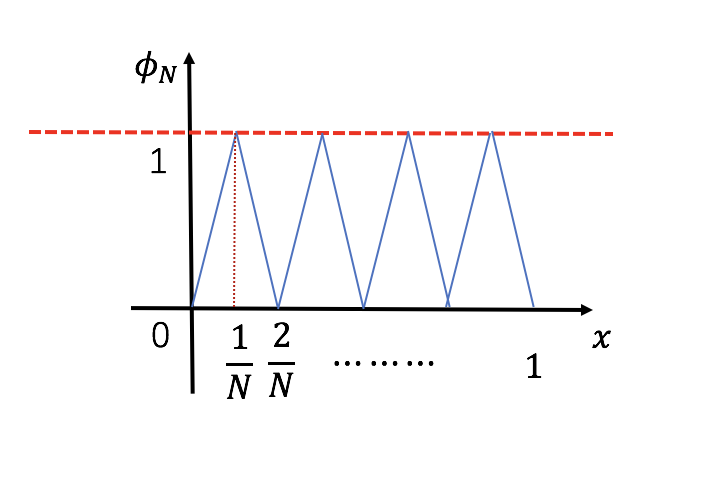
\includegraphics[width=6cm]{week4/4_3.png}
\caption{Plot of function $\phi_N(x)$}
\end{figure}
As we can see, $N$ is the maximum slope of the piecewise linear function $\phi_N$.
\item
Let $M$ be the maximum slope of the piecewise linear function $f$, and pick a positive even integer $m$ such that
\[
\frac{1}{2}mN\varepsilon>M+n.
\]
Then we construct function
\[
g(x) = f(x)+\frac{1}{2}\varepsilon\phi_{mN}(x)
\]
As we can see, $d(f,g)=\frac{1}{2}\varepsilon<\varepsilon$, thus $g\in B(f,\varepsilon).$ Also note that
\begin{align*}
\left|\frac{g(x+h)-g(x)}{h}\right|
&\ge
\left|\frac{1/2\varepsilon(\phi_{mN}(x+h) - \phi_{mN}(x))}{h}\right|
-
\left|\frac{f(x+h)-f(x)}{h}\right|\\
&\ge
\frac{1}{2}\varepsilon\left|\frac{(\phi_{mN}(x+h) - \phi_{mN}(x))}{h}\right|-M\\
&=\frac{1}{2}mN\varepsilon - M>n
\end{align*}
for $x$ in $(0,1-\frac{1}{mN})$ and some $h\in(0,1-x)$. Hence, $g\notin E_n$. The proof is complete.
\end{itemize}
\end{proof}

\subsection{Continuity Analysis}
Recall the definition for continuity:
\begin{itemize}
\item
A function $f$ is said to be continuous at $x_0\in I$ if $\forall\varepsilon>0$, there exists $\delta>0$ ($\delta$ depends on $x_0$ and $\varepsilon$) such that
\[
\begin{array}{ll}
|f(x) - f(x_0)|<\varepsilon,
&
\forall|x-x_0|<\delta
\end{array}
\]
\item
A function $f$ is continuous on $I$ if it is continuous at every point in $I$.
\end{itemize}
\begin{definition}[Uniform]
We say $f$ is \emph{uniformly continuous} on $I$ if $\forall\varepsilon>0$, there exists $\delta$ (depend only on $\varepsilon$, but independent of $x\in I$) such that
\[
|f(y)-f(x)|<\varepsilon,\mbox{ if }|x-y|<\delta
\]
\end{definition}
\begin{remark}
It is useful to note that the uniform continuity places a upper bound on the growth of the function at every point, i.e., the function cannot grow too fast.
\end{remark}
\begin{example}
Given a function $f(x)=x^2$,
\begin{enumerate}
\item
Is it uniformly continuous on $[0,1]$?

Yes, intuitively the growth of $x^2$ is limited within bounded interval.
\item
Is it uniformly continuous on $\mathbb{R}$?

No, intuitively the growth of $x^2$ tends to infinite as $x\to\infty$.

\textbf{Proof:} For fixed $x$, if $|y-x|<\delta$, if we choose $|x|\ge\frac{\varepsilon}{2\delta}+\frac{\delta}{2}$, then
\begin{align*}
\underbrace{|f(y) - f(x)|}_{\varepsilon} &= |y^2 - x^2| = |y+x|\underbrace{|y - x|}_{\delta}\\
&\ge (|2x| - |x-y|)|y - x|\ge(\frac{\varepsilon}{\delta}+\delta-\delta)\delta=\varepsilon
\end{align*}
which is a contradiction.
\end{enumerate}
\end{example}
%
%\begin{definition}[Lipschitz]
%
%\end{definition}
%
%
%\begin{definition}[Holder]
%
%\end{definition}
\begin{figure}[H]
\centering

\includegraphics[width=8cm]{week4/4_2.jpeg}
\caption{The proof and application for the Theorem(\ref{The:4:2}) is Mandatory. If you don't know how to do it in the exam, Prof.Ni will fail you without hesitation.}
\end{figure}
\begin{theorem}\label{The:4:2}
Suppose that $f$ is continuous on a compact set $D$. Then $f$ is uniformly continuous on $D$.
\end{theorem}
\begin{proof}
For given $\varepsilon>0$, since $f$ is continuous at $x$, there exists $\delta_x>0$ s.t.
\[
\begin{array}{ll}
|f(y)-f(x)|<\frac{\varepsilon}{2},
&
\mbox{if }|y-x|<\delta_x.
\end{array}
\]
Construct an open cover $\{B_{\delta_x}(x)\mid x\in D\}$ of $D$ with
\[
B_{\delta_x}(x) = \{y\in D\mid |y-x|<\frac{1}{2}\delta_x\}.
\]
The set $D$ is compact implies there exists a finite subcover:
\begin{equation}
D\subseteq B_{\delta_{x_1}}(x_1)\bigcup 
B_{\delta_{x_2}}(x_2)\bigcup\cdots\bigcup
B_{\delta_{x_k}}(x_k).\label{Eq:4:1}
\end{equation}
Construct $\delta>0$ such that $B_\delta(x)$ must be contained entirely in one of the ball, say $B_{\delta_{x_j}}(x_j)$ (Exercise $\#7$)

Therefore given $|y-x|<\delta$ we imply $x,y\in B_{\delta_{x_j}}(x_j)$ for some $j$, which follows that
\[
|f(y) - f(x)| \le |f(y) - f(x_j)|+|f(x_j) - f(x)|<\frac{\varepsilon}{2}+\frac{\varepsilon}{2}=\varepsilon
\]
\end{proof}
\paragraph{Verification of Exercise}
Such a $\delta$ is constructed as
\[
\delta=\frac{1}{2}\min\{\delta_{x_1},\delta_{x_2},\dots,\delta_{x_k}\}.
\]
Thus for any $x,y$ with $|y-x|<\delta$, by(\ref{Eq:4:1}), there exists $j$ such that $x\in B_{\delta_{x_j}}(x_j)$, and hence
\begin{equation}
|x -x_j|<\frac{1}{2}\delta_{x_j}
\end{equation}
Also, we have
\begin{equation}
|y-x_j|\le|y-x|+|x-x_j|\le\delta + \frac{1}{2}\delta_{x_j}\le\delta,
\end{equation}
i.e., $y$ is also in $B_{\delta_{x_j}}(x_j)$.





\begin{definition}[Convex]
A real-valued function $f$ defined in $(a,b)$ is said to be convex if 
\[
f(tx+(1-t)y)\le tf(x)+(1-t)f(y)
\]
whenever $a<x<b,a<y<b,0<t<1$.
\end{definition}
Check Rudin's book for the proof that a convex function is always continuous.



%
%\begin{definition}[Monotone]
%
%\end{definition}

















